\documentclass[12pt,oneside,titlepage]{scrartcl} 

\newcommand{\myAutor}{Rico  (Matrikelnummer 12345)\\ \> \> \> 
Henning   (Matrikelnummer 12345)\\ \> \> \> 
Julian  (Matrikelnummer 12345)} % Autor
\newcommand{\myAdresse}{Stra\ss e 123 \\ \> \> \> 57xxx Siegerland} % Adresse
\newcommand{\myTitel}{Browser RPG-Adventure } % Titel der Arbeit
\newcommand{\myBetreuer}{Daniel Bitzer} % Betreuer
\newcommand{\myLehrveranstaltung}{Web Technologie} % Lehrveranstaltung
\newcommand{\myMatrikelNr}{123456} % Matrikelnummer
\newcommand{\myOrt}{Siegen} % Ort
\newcommand{\myAbgabeDatum}{\today} % Datum der Abgabe
\newcommand{\mySemesterZahl}{5} % Semesterzahl
\newcommand{\myHochschulName}{FOM Hochschule für Oekonomie \& Management Essen} % Name der Hochschule
\newcommand{\myHochschulStandort}{Siegen} % Standort der Hochschule
\newcommand{\myStudiengang}{Wirtschaftsinformatik} % Studiengang
\newcommand{\myThesisArt}{Seminararbeit als Projektdokumentation} % Art der Arbeit
\newcommand{\myAkademischerGrad}{Bachelor of Science (B. Sc.)} % Zu erlangender akademische Grad
\newcommand{\myFirma}{Mustermann GmbH} % Firma

\usepackage[ngerman]{babel}
\selectlanguage{ngerman}
\usepackage[babel,german=quotes]{csquotes}

\usepackage[utf8]{luainputenc}
\usepackage[T1]{fontenc}
\usepackage{fancyhdr}
\usepackage{fancybox}
\usepackage[a4paper, left=4cm, right=2cm, top=4cm, bottom=2cm]{geometry}
\usepackage{graphicx}
\usepackage{colortbl}
\usepackage[capposition=top]{floatrow}
\usepackage{array}
\usepackage{float}      %Positionierung von Abb. und Tabellen mit [H] erzwingen
\usepackage{footnote}
\usepackage[singlelinecheck=false, labelfont=bf, font=bf]{caption} % Tabellendesign lt. Leitfaden
\usepackage{caption}
\usepackage{enumitem}
\usepackage{amssymb}
\usepackage{mathptmx}
\usepackage[scaled=0.9]{helvet} 
\usepackage{courier}
\usepackage{amsmath}
\usepackage[table]{xcolor}
\usepackage{marvosym}			% Verwendung von Symbolen, z.B. perfektes Eurozeichen
\usepackage[colorlinks=true,linkcolor=black]{hyperref}
\definecolor{darkblack}{rgb}{0,0,0}
\hypersetup{colorlinks=true, breaklinks=true, linkcolor=darkblack, menucolor=darkblack, urlcolor=darkblack}
\renewcommand\familydefault{\sfdefault}
\usepackage{ragged2e}

\usepackage[hang, multiple]{footmisc} % Mehrere Fussnoten nacheinander mit Komma separiert
\setlength{\footnotemargin}{1em}

%\usepackage{todonotes} % todo Aufgaben als Kommentare verfassen für verschiedene Editoren

\usepackage{epstopdf} %Pakete für Tabellen
\usepackage{nicefrac} % Brüche
\usepackage{multirow}
\usepackage{rotating} % vertikal schreiben
\usepackage{mdwlist}
\usepackage{tabularx}% für breitenangabe

\definecolor{dunkelgrau}{rgb}{0.8,0.8,0.8}
\definecolor{hellgrau}{rgb}{0.0,0.7,0.99}
% Colors for listings
\definecolor{mauve}{rgb}{0.58,0,0.82}
\definecolor{dkgreen}{rgb}{0,0.6,0}

\usepackage{listings} % sauber formatierter Quelltext
% JavaScript als Sprache definieren:
\lstdefinelanguage{JavaScript}{
	keywords={break, super, case, extends, switch, catch, finally, for, const, function, try, continue, if, typeof, debugger, var, default, in, void, delete, instanceof, while, do, new, with, else, return, yield, enum, let, await},
	keywordstyle=\color{blue}\bfseries,
	ndkeywords={class, export, boolean, throw, implements, import, this, interface, package, private, protected, public, static},
	ndkeywordstyle=\color{darkgray}\bfseries,
	identifierstyle=\color{black},
	sensitive=false,
	comment=[l]{//},
	morecomment=[s]{/*}{*/},
	commentstyle=\color{purple}\ttfamily,
	stringstyle=\color{red}\ttfamily,
	morestring=[b]',
	morestring=[b]"
}

\lstset{
	%language=JavaScript,
	numbers=left,
	numberstyle=\tiny,
	numbersep=5pt,
	breaklines=true,
	showstringspaces=false,
	frame=l ,
	xleftmargin=5pt,
	xrightmargin=5pt,
	basicstyle=\ttfamily\scriptsize, 
	stepnumber=1,
	keywordstyle=\color{blue},          % keyword style
  	commentstyle=\color{dkgreen},       % comment style
  	stringstyle=\color{mauve}         % string literal style
}

\usepackage[
    style           = apa6, 
    uniquelist      = false,    
    maxcitenames    = 6,
    backend         = biber,
	urldate         = short,
	uniquename 		= true,
	language		= ngerman
	]{biblatex} 
		
	%% START Block für Funktion (1. Nennung von 2-6 Autoren: Alle Namen, danach nur noch 1. Name + et.al) 
	\usepackage{lmodern} 
	\makeatletter
	\newcommand{\apamaxcitenames}{6}
	\DeclareNameFormat{labelname}{%
	  \ifthenelse{\value{uniquelist}>1}
		{\numdef\cbx@min{\value{uniquelist}}}
		{\numdef\cbx@min{\value{minnames}}}%
	  \ifboolexpr{test {\ifnumcomp{\value{listcount}}{=}{1}}
				  or test {\ifnumcomp{\value{listtotal}}{=}{2}}}
		{\usebibmacro{labelname:doname}%
		  {\namepartfamily}%
		  {\namepartfamilyi}%
		  {\namepartgiven}%
		  {\namepartgiveni}%
		  {\namepartprefix}%
		  {\namepartprefixi}%
		  {\namepartsuffix}%
		  {\namepartsuffixi}}
		{\ifboolexpr{test {\ifnumcomp{\value{listtotal}}{>}{\apamaxcitenames}}
					 or test {\ifciteseen}}
		 {\ifnumcomp{\value{listcount}}{<}{\cbx@min + 1}
		   {\usebibmacro{labelname:doname}%
			 {\namepartfamily}%
			 {\namepartfamilyi}%
			 {\namepartgiven}%
			 {\namepartgiveni}%
			 {\namepartprefix}%
			 {\namepartprefixi}%
			 {\namepartsuffix}%
			 {\namepartsuffixi}}
		   {}%
		  \ifnumcomp{\value{listcount}}{=}{\cbx@min + 1}
			{\ifnumcomp{\value{listcount}}{<}{\value{listtotal}}
			  {\printdelim{andothersdelim}\bibstring{andothers}}
			  {\usebibmacro{labelname:doname}%
				{\namepartfamily}%
				{\namepartfamilyi}%
				{\namepartgiven}%
				{\namepartgiveni}%
				{\namepartprefix}%
				{\namepartprefixi}%
				{\namepartsuffix}%
				{\namepartsuffixi}}}
			{}%
		  \ifnumcomp{\value{listcount}}{>}{\cbx@min + 1}
		   {\relax}%
		   {}}%
		 {\usebibmacro{labelname:doname}%
		   {\namepartfamily}%
		   {\namepartfamilyi}%
		   {\namepartgiven}%
		   {\namepartgiveni}%
		   {\namepartprefix}%
		   {\namepartprefixi}%
		   {\namepartsuffix}%
		   {\namepartsuffixi}}}}
	\makeatother 
	\DeclareLanguageMapping{ngerman}{ngerman-apa}
	%% ENDE Block für Funktion (1. Nennung von 2-6 Autoren: Alle Namen, danach nur noch 1. Name + et.al)
	
	\DeclareDelimFormat*{finalnamedelim}{\addspace\bibstring{and}\space} % In Parencite von "&" auf "und" ändern
	\hypersetup{hidelinks}  %Grüne Links auf Literaturverz. unterdrücken.
	\setlength\bibitemsep{1.3ex} % Abstände im Literaturverzeichnis erhöhen
	\setlength\bibnamesep{1.0ex}
	\AtBeginBibliography{\singlespacing} % Zeilenabstand im Literaturverzeichnis ist Einzeilig - siehe Leitfaden S. 14
	\urlstyle{same} %Standard-Font für Link anstelle der "Schreibmaschinenschrift"
	\DeclareFieldFormat[misc]{urldate}{[#1\printfield{urldate}].} 	% Anpassung @online + @misc Bibl: Datum in eckigen Klammern ans Ende
	\DeclareFieldFormat[misc]{title}{\mkbibemph{#1}} %Anpassung @online + @misc Titel Kursiv	
	\DeclareFieldFormat[misc]{url}{Verfügbar unter\space \url{#1}} 	%Anpassung @online + @misc Text vor URL
	\renewbibmacro*{url+urldate}{\usebibmacro{url}\setunit{\addspace}\usebibmacro{urldate}}  % URL vor Abrufdatum setzen + getrennte Wörter "Verfügbar" und "Unter" entfernen
%%%% APA ENDE

\addbibresource{literatur.bib} %Bib-Datei einbinden
%\nocite{*} % Die folgende Zeile trägt ALLE Werke aus literatur.bib in das Verz. ein, auskommentieren um nur die anzuzeigen, die zitiert wurden


\usepackage{hyphsubst} %Silbentrennung
\HyphSubstIfExists{ngerman-x-latest}{%
\HyphSubstLet{ngerman}{ngerman-x-latest}}{}

\graphicspath{{./}{./media/}} % Pfad fuer Abbildungen

\usepackage{titletoc} % Weitere Ebene einfügen
\makeatletter

% Setze die Tiefe des Inhaltsverzeichnis auf 4 Ebenen -  Damit erscheinen \paragraph-Sektionen auch im Inhaltsverzeichnis
\setcounter{secnumdepth}{4}
\setcounter{tocdepth}{2}

% Fuege Abstand nach unten wie in einer normalen \section hinzu
\renewcommand{\paragraph}{%
  \@startsection{paragraph}{4}%
  {\z@}{3.25ex \@plus 1ex \@minus .2ex}{1.5ex plus 0.2ex}%
  {\normalfont\normalsize\bfseries\sffamily}%
}

\makeatother

\usepackage{appendix} % Paket für die Nutzung von Anhängen
\usepackage{setspace} % Zeilenabstand 1,5-zeilig
\onehalfspacing

\setlength{\parindent}{0mm} % Absätze durch eine neue Zeile
\setlength{\parskip}{0.8em plus 0.5em minus 0.3em}

\sloppy					%Abstände variieren
\pagestyle{headings}

\usepackage[printonlyused]{acronym} % Abkürzungsverzeichnis


% PDF Meta Daten setzen
\hypersetup{
    pdfinfo={
        Title={Nutzbarkeit und Effizienz von smarten Displays - Ein Proof of Conept in Quartieren der Wohnungswirtschaft},
        Subject={\myStudiengang},
        Author={\myAutor},
        Build=1.1
    }
}

% Umlaute in Code korrekt darstellen - siehe  https://en.wikibooks.org/wiki/LaTeX/Source_Code_Listings
\lstset{literate=
	{á}{{\'a}}1 {é}{{\'e}}1 {í}{{\'i}}1 {ó}{{\'o}}1 {ú}{{\'u}}1
	{Á}{{\'A}}1 {É}{{\'E}}1 {Í}{{\'I}}1 {Ó}{{\'O}}1 {Ú}{{\'U}}1
	{à}{{\`a}}1 {è}{{\`e}}1 {ì}{{\`i}}1 {ò}{{\`o}}1 {ù}{{\`u}}1
	{À}{{\`A}}1 {È}{{\'E}}1 {Ì}{{\`I}}1 {Ò}{{\`O}}1 {Ù}{{\`U}}1
	{ä}{{\"a}}1 {ë}{{\"e}}1 {ï}{{\"i}}1 {ö}{{\"o}}1 {ü}{{\"u}}1
	{Ä}{{\"A}}1 {Ë}{{\"E}}1 {Ï}{{\"I}}1 {Ö}{{\"O}}1 {Ü}{{\"U}}1
	{â}{{\^a}}1 {ê}{{\^e}}1 {î}{{\^i}}1 {ô}{{\^o}}1 {û}{{\^u}}1
	{Â}{{\^A}}1 {Ê}{{\^E}}1 {Î}{{\^I}}1 {Ô}{{\^O}}1 {Û}{{\^U}}1
	{œ}{{\oe}}1 {Œ}{{\OE}}1 {æ}{{\ae}}1 {Æ}{{\AE}}1 {ß}{{\ss}}1
	{ű}{{\H{u}}}1 {Ű}{{\H{U}}}1 {ő}{{\H{o}}}1 {Ő}{{\H{O}}}1
	{ç}{{\c c}}1 {Ç}{{\c C}}1 {ø}{{\o}}1 {å}{{\r a}}1 {Å}{{\r A}}1
	{€}{{\EUR}}1 {£}{{\pounds}}1 {„}{{\glqq{}}}1
}

\pagestyle{fancy} % Kopfbereich / Header definieren
\fancyhf{} % Seitenzahl oben, mittig, mit Strichen beidseits: \fancyhead[C]{-\ \thepage\ -}

\fancyhead[C]{\thepage} % Seitenzahl oben, mittig, entsprechend Leitfaden ohne Striche beidseits
\renewcommand{\headrulewidth}{0.4pt} % Waagerechte Linie unterhalb des Kopfbereiches anzeigen. Alternativ weg: \renewcommand{\headrulewidth}{0pt}

\begin{document} % Start the document here

\pagenumbering{Roman}								% Seitennumerierung auf römisch umstellen
\renewcommand{\refname}{Literaturverzeichnis}		% "Literatur" in "Literaturverzeichnis" umbenennen
\newcolumntype{C}{>{\centering\arraybackslash}X}	% Neuer Tabellen-Spalten-Typ: Zentriert und umbrechbar

\begin{titlepage} % Titlepage/Deckblatt
	\newgeometry{left=2cm, right=2cm, top=2cm, bottom=2cm}
	\begin{center}
		\textbf{\myHochschulName}\\
		\textbf{Hochschulzentrum \myHochschulStandort}\\
		\vspace{1.5cm}
			
\includegraphics[width=3cm]{media/fomLogo} \\
		\vspace{1.5cm}
		Berufsbegleitender Studiengang\\
		\myStudiengang, \mySemesterZahl. Semester\\
		\vspace{2cm}
		\textbf{\myThesisArt}\\
		%\textbf{zur Erlangung des Grades eines	}\\
		%\textbf{\myAkademischerGrad}\\
		% Oder für Hausarbeiten:
		\textbf{im Rahmen der Lehrveranstaltung}\\
		\textbf{\myLehrveranstaltung}\\
		\vspace{2cm}
		über das Thema\\
		\Large{\myTitel}\\
		\vspace{0.2cm}
	\end{center}
	\normalsize
	\vfill
	\begin{tabbing}
		Links \= Mitte \=Mittez \= Rechts\kill
		Betreuer: \> \> \>\myBetreuer\\
		\> \> \\
		Autoren: \> \> \> \myAutor\\
		%\> \> \>  Matrikelnummer: \myMatrikelNr\\
		%\> \> \> \myAdresse\\
		\> \> \>  \\
		Abgabe: \> \> \> \myAbgabeDatum
	\end{tabbing}
\end{titlepage}

%-------Ende Titelseite-------------


% Sperrvermerk
%\newpage
%\thispagestyle{empty}
%\section*{Sperrvermerk}
%Die vorliegende Abschlussarbeit mit dem Titel \enquote{\myTitel} enthält unternehmensinterne Daten der Firma \myFirma . Daher ist sie nur zur Vorlage bei der FOM sowie den Begutachtern der Arbeit bestimmt. Für die Öffentlichkeit und dritte Personen darf sie nicht zugänglich sein.
%\par\medskip
%\par\medskip
%\_\_\_\_\_\_\_\_\_\_\_\_\_\_\_\_\_\_\_\_\_\_\_\_ \hspace{1.5cm} \_\_\_\_\_\_\_\_\_\_\_\_\_\_\_\_\_\_\_\_\_\_\_\_ \\
%(Ort, Datum)\hspace{4.5cm}
%(Eigenhändige Unterschrift)
%\newpage

% 
% Inhaltsverzeichnis
\setcounter{page}{2}
\addtocontents{toc}{\protect\enlargethispage{-20mm}}
\clearpage
\tableofcontents
\newpage
\setcounter{tocdepth}{2} %wurde  in zusaetzlichesMaterial.tex auf 0 gesetzt um Inhalt des Anhangs zu verbergen. Dadurch gehen allerdings Abbildungs und Tabellenverzeichnis kaputt.

%\addcontentsline{toc}{section}{Abbildungsverzeichnis} % Falls das Abkürzungsverzeichnis im Inhaltsverzeichnis angezeigt werden 
%\section*{Abbildungsverzeichnis} % Abbildungsverzeichnis
\listoffigures % Abbildungsverzeichnis
\newpage

%\addcontentsline{toc}{section}{Tabellenverzeichnis} % Falls das Abkürzungsverzeichnis im Inhaltsverzeichnis angezeigt werden 
%\section*{Tabellenverzeichnis} % Tabellenverzeichnis
\listoftables % Tabellenverzeichnis
\newpage

%\addcontentsline{toc}{section}{Abkürzungsverzeichnis} % Falls das Abkürzungsverzeichnis im Inhaltsverzeichnis angezeigt werden soll einkommentieren.
\section*{Abkürzungsverzeichnis} % Abkürzungsverzeichnis

\begin{acronym}[WoWi]\itemsep0pt %der Parameter in Klammern sollte die längste Abkürzung sein. Damit wird der Abstand zwischen Abkürzung und Übersetzung festgelegt
	\acro{PoC}{Proof of Concept}
	\acro{WoWi}{Wohnungswirtschaft}
\end{acronym}
\newpage

\pagenumbering{arabic} % Seitennummerierung auf arabisch und ab 1 beginnend umstellen
\setcounter{page}{1}








\section{Aufgabenbeschreibung}
Beispielinhalt und Texte:
Das Thema der Seminararbeit gründet als Idee vor allem aus den folgenden beiden Beobachtungen aus privatem Lebensalltag und beruflicher Praxis: 
\begin{enumerate}
	\item Die seit den 2010er Jahren aufkommenden \textbf{smarten Technologien} finden im öffentlichen Raum und im Lebensalltag breiter Bevölkerungsschichten immer mehr Einzug. Drei Anwendungsbeispiele verdeutlichen und belegen das: 
	\begin{itemize}
	 \item Smart Watch: Uhren die z.B. um Fitness- und Nachrichtenfunktionen erweitert sind.
	 \item Smart TV: Fernsehgeräte die z.B. Zugriff auf Internet-Mediatheken erlauben.
	 \item Smart Home: Hausautomatisierungen und -steuerungen im privaten Bereich für  z.B. Licht und Heizung.
	 \end{itemize}

	 \item Das Aufkommen und der Erfolg der \textbf{PropTech\footnote{Kofferwort, englisch, aus 'property' (Immobilien) und 'technology' (Technologiegen)}-Branche} sowie die dieser Branche zuzuordnenden Unternehmen belegt die Relevanz von Innovation für die Wohnungswirtschaft ebenso wie die folgenden Erkenntnisse einer Studie \parencite[S. 18]{zia}:
	 \begin{itemize}
		 \item 72\% der befragten immobilienwirtschaftlichen Unternehmen nehmen Effizienzsteigerungen in Kernprozessen durch Einsatz digitaler Technologien an.
		 \item Weiter: Über ein Drittel gehen davon aus, dass Neugeschäft durch Einsatz digitaler Technologien generiert werden kann. 
	 \end{itemize}
\end{enumerate}

Vorgenannte Beobachtungen führen zu folgender Hypothese:

 \Rightarrow \textbf{Der Einsatz von smarten Displays in Quartieren der \ac{WoWi} ist möglich, wirtschaftlich und innovativ.}



\subsection{Was ist das Ziel der Projektarbeit?}
Beispielinhalt und Texte:
Als mögliche Standorte ergeben sich in Anlehnung an bisher übliche \glqq{}schwarze Bretter\grqq{} und \glqq{}Schaukästen\grqq{} in den Gebäuden sowie auch im Außenbereich vorhandenen Anlagen (Schaukästen, Werbeanlagen) auch für smarte Displays einige Vor- und Nachteile (Pro und Contra) die wie folgt stichpunktartig beschrieben werden: 

 \begin{itemize}
	 \item \textbf{Innenbereich:} 
	 \\ Wandmontage ebenso wie üblich und bekannte Schaukästen und schwarze Bretter im Windfang oder dem Etagenflur im Erdgeschoss eines Mietshauses.\\
	 \textbf{Pro:}\\
	  - Weiternutzung vorhandener, bewährter Montageorte \\
	  - Baurechtlich genehmigungsfrei \\
	  - Anbindung an Strom und Internet leichter als im Außenbereich \\
	  - Günstigere Bauart (kann weniger witterungsfest und vandalismussicher sein)\\
	 \textbf{Contra:}\\
	  - Wird wenig innovative Bauart zur Folge haben\\
	  - Kleinere Anzeigeflächen \\
	  - Nutzerkreis umfasst nur Mieter und Besucher des Hauses
	 \item \textbf{Außenbereich:} 
	 \\ Als freistehende Installation vor einem Wohngebäude, an einem markanten Wegepunkt im Quartier oder einem Innenhof eines Gebäudekomplexes.\\
	 \textbf{Pro:}\\
	  - Höhere Sichtbarkeit und Reichweite (nicht nur Mieter und Besucher eines Hauses, sondern auch Umfeld, Nachbarn und Durchgangsverkehr)  \\
	  - Attraktive Bauarten möglich \\
	  - Eröffnet weitergehende Nutzungsmöglichkeiten \\
	 \textbf{Contra:}\\
	  - Höhere Investitionskosten durch dem Standort geschuldete Bauart und Größe \\
	  - Erdarbeiten werden in der Regel nötig sein (Stromanschluss)  \\
	  - Baurechtlich genehmigungspflichtig, verursacht Mehrkosten und Aufwand
	  \item \textbf{Übergangsbereich Hauseingangstüre:} 
	  \\ Anbringung an Flächen die das Gebäude und den Außenbereich verbinden, beispielhaft genannt hier: Seitenteil der Türelemente im Hauseingangsbereich.\\
	  \textbf{Pro:}\\
	   - Unter Umständen umsetzbar als Modernisierungsmaßnahme (Nutzung als Videogegensprechanlage)  \\
	   - Technikaverse Bewohner und Besucher kommen zwangläufig in Kontakt mit dem smart Display \\
	  \textbf{Contra:}\\
	   -  Vorteile ergeben sich z.T. nur in noch nicht modernisiertem Bestand \\
	   -  Kleinerer Nutzerkreis und Anzeigefläche \\
 \end{itemize}

Eine weitergehende Bewertung oder Befürwortung einzelner Standorte soll hier nicht erfolgen um einzelne Anwendungsfälle nicht hier schon auszuschließen.


\subsection{Worin bestehen die (wahrscheinlichen) Herausforderungen? (allg. technisch und auch persönlich)}
Beispielinhalt und Texte:
Der Begriff soll daher hier geschärft werden um in der weiteren Verwendung un­miss­ver­ständ­lich zu sein.  

Die Definition erfolgt unter Bezug auf
\begin{enumerate}
	\item  die erfolgte Abgrenzung in 'enge' und 'weite' Definition nach \citeauthor{wirtschaftsfaktorimmo} (\citeyear[S. 9]{wirtschaftsfaktorimmo}) sowie
	\item die institutionelle Systematisierung der Immobilienwirtschaft nach \citeauthor{brauer2011einfuhrung} (\citeyear[S. 26]{brauer2011einfuhrung}).
\end{enumerate}

Die daraus entnommenen Zitate sollen hier im weiteren als gültige Definition für den verwendeten Begriff \textbf{Wohnungswirtschaft (WoWi)} gelten:  
\begin{itemize}
	\item Aus \citeauthor{wirtschaftsfaktorimmo} (\citeyear[S. 9]{wirtschaftsfaktorimmo}): \glqq{}alle Unternehmen, die an der Bewirtschaftung, Vermittlung und Verwaltung von Immobilien unmittelbar beteiligt sind\grqq{}. 
	 \item Sowie nach \citeauthor{brauer2011einfuhrung} (\citeyear[S. 36]{brauer2011einfuhrung}) zu den unterschiedlichen Rechtsformen \glqq{}(...)kommunalen, genossenschaftlichen und privaten Unternehmen(...)\grqq{} und den gleichwohl identischen Aufgabenfeldern: \glqq{}(...)nachhaltige Vermietung und Bestandsmanagement(...)\grqq{}.
\end{itemize}





\newpage
\section{Anforderungen}
Beispielinhalt und Texte:
Die genaue Zuordnung stellt sich also wie folgt dar:

\begin{table}[H]
	\caption{Zuordnung der Anforderungen der Hypothese zu den kritischen Anforderungen des Proof of Concept (PoC)}
	\label{tbl:zuordnungHypothesePoc}
	\begin{tabularx}{\textwidth}[ht]{|l|c|X|}
	\hline
	\textbf{Anforderung der Hypothese} & \textbf{Zuordnung} & \textbf{Abbildung in \ac{PoC}} \\
	\hline\hline 
	ist möglich & \Leftrightarrow & Prüfung der Machbarkeit  \\
	\hline 
	ist wirtschaftlich & \Leftrightarrow &  Effizienz-Faktoren aufzeigen \\
	\hline 
	ist innovativ & \Leftrightarrow &  Nutzbarkeit und Anwendungsfälle \\
	\hline
	\end{tabularx}
\end{table}


\subsection{Welche Techniken/ Technologien sollen eingesetzt werden, um die Aufgabe zu lösen/ realisieren?}
Beispielinhalt und Texte:

Eine Betrachtung der Wirtschaftlichkeit einer Einzelinvestition in ein smart Display in einem Quartier könnte damit nach z.B. folgendem Schema erfolgen:


\begin{table}[H]
	\caption{Mögliches Schema einer Wirtschaftlichkeits- und Effizienzbetrachtung der Einzelinvestition in smart Displays}
	\label{tbl:SchemaWBsmartDisplay}
	\begin{tabularx}{\textwidth}[ht]{cl}
	\hline
	\textbf{ - }   &  Investitionskosten (der Einzelmaßnahme) \\
	\textbf{ - }   &  lfd. Betriebs- und Wartungskosten  \\
	\textbf{ + }   &  lfd. Einsparung Personalkosten  \\
	\textbf{ + }   &  Refinanzierung als Modernisierungsmaßnahme   \\
	\textbf{ + }   &  Umlage von (Teilen der) Betriebskosten auf Gebäudenutzer  \\
	\textbf{ + }   &  Mehrerlöse durch Überlassung als Werbefläche an Dritte  \\
	\hline\hline
	\textbf{ = }   &  \textbf{in Euro messbare Wirtschaftlichkeit} \\
	\textbf{ + }   &  Digitalisierung eines Geschäftsprozesses  \\
	\textbf{ + }   &  Imagegewinn für das Quartier \\
	\textbf{ + }   &  Öffentlichkeitswirksame Einführung und Realisierung  \\
	\hline\hline
	\textbf{ = }   &  \textbf{gesamt zu bewertende Effizienz} \\
	\hline
\end{tabularx}
\end{table}

Kommt man nun zurück auf die Definition des Bergriffs der Effizienz nach \citeauthor{eichhorn2016} (\citeyear[S. 183 f.]{eichhorn2016}), kann man feststellen, dass es für die Beurteilung wesentliche Faktoren gibt, die nicht der Wirtschaftlichkeit zuzurechnen sind.



\subsection{Warum sollen gerade diese eingesetzt werden?}
Beispielinhalt und Texte:
Mit smarten Displays sind in dieser Seminararbeit nicht die von Desktop-Computer abnehmbaren und tragbaren LCD-Monitore gemeint die 2002 im Zusammenhang mit Microsofts Betriebssystem \glqq{}Windows CE for Smart Displays\grqq{} vorgestellt wurden \parencite{heise-ms-sd} und im Jahr 2004 wieder eingestellt worden sind \parencite{ct-3-2004}. 

\begin{figure}[H]
	\caption{Handteil eines smart Displays nach Microsoft-Konzept}\label{fig:HandteilMSsmartDisplay}
	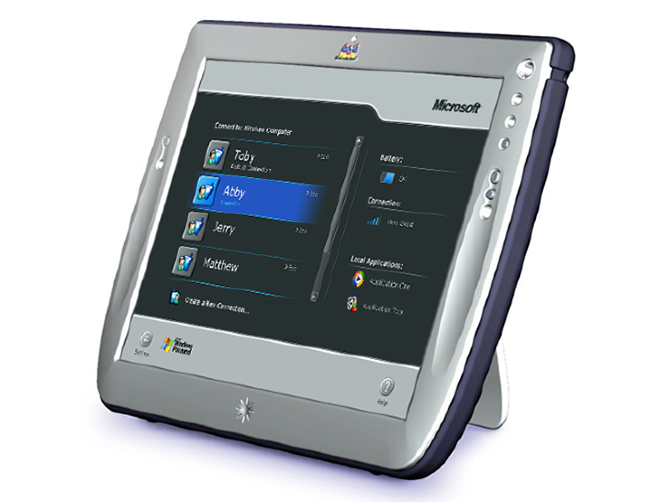
\includegraphics[height=5cm,keepaspectratio]{mira}
	\\
	Quelle: Homepage von Mark Strehlow, Senior Interaction Designer\\ im Projekt Mira (\href{https://msdo.us/Microsoft-Mira}{msdo.us/Microsoft-Mira})
\end{figure}

Vielmehr sind hier erst noch durch Forschung und Entwicklung für die \ac{WoWi} zu schaffenden und nutzbar zu machenden Geräte gemeint.


\subsection{Gibt es besondere Anforderungen? (technisch, Benutzer, sonstige)}
Beispielinhalt und Texte:

\newpage
\section{Herangehensweise}
Beispielinhalt und Texte:

\subsection{Wie soll das Ziel erreicht werden (Vorgehen, Architektur)}
Beispielinhalt und Texte:

\newpage
\section{Vorstellung des Ergebnisses}
Beispielinhalt und Texte:

\newpage
\section{Reflektion}
Beispielinhalt und Texte:

 die Anwendung wird hier durch eine Betrachtung  der untenstehenden Punkte erfolgen: 
\begin{itemize}
	\item \textbf{Prüfung rechtlicher und IT-technischer Machbarkeit:}
	\\ Neben baurechtlicher Betrachtung hier auch Prüfung in Bezug auf verschiedenartige Realisierungen in Größe, Standort, Bauart und IT-Integration.
	\item \textbf{Aufzeigen und erörtern relevanter Effizienz-Faktoren:}
	\\ Umfasst typisch erwartbare Effizienz-Faktoren wie die Wirtschaftlichkeit ebenso wie auch darüber hinausgehende Auswirkungen die zur ebenso zur Effizienz zu zählen sind.
	\item \textbf{Darstellung möglicher Nutzbarkeiten und Anwendungsfälle:}
	\\ Ausführungen zu erwartbaren Einflüssen auf vorhandene Geschäftsprozesse in der \ac{WoWi} aber auch durch Aufzeigen von neuartigen und darüber hinausgehenden Anwendungsfällen und -bereichen.
\end{itemize}

Diese drei vorgenannten Punkte spiegeln die drei Anforderungen aus der Hypothese der Einleitung wieder und entsprechen dieser genau, in den jeweils genannten Reihenfolgen. 





















\newpage % Literaturverzeichnis

% Im Literaturverzeichnis "und" wieder durch "&" ersetzen	
	\DeclareDelimFormat*{finalnamedelim}{\addspace\&\space}

% Punkt hinter und vor der Jahreszahl entfernen	- Wichtig für Quell-Arten wie misc und online -- Sonst ein überflüssiger Punkt im LitVerz.
	\renewbibmacro*{author}{%
	\printtext{%
	\ifnameundef{author}
	{\usebibmacro{labeltitle}}
	{\printnames[apaauthor][-\value{listtotal}]{author}%
	\setunit*{\addspace}%
	\printfield{nameaddon}%
	\ifnameundef{with}
	{}
	{\setunit{}\addspace\mkbibparens{\printtext{\bibstring{with}\addspace}%
	\printnames[apaauthor][-\value{listtotal}]{with}}
	\setunit*{\addspace}}}%
	% \newunit\newblock%
	\usebibmacro{labelyear+extradate}}}

\printbibliography[heading=bibintoc,title=Literaturverzeichnis]

\newpage % Ehrenwörtliche Erklärung
\pagenumbering{gobble} % Keine Seitenzahlen mehr
\section*{Ehrenwörtliche Erklärung} 
	Hiermit versichere ich, dass die vorliegende Arbeit von mir selbstständig und ohne unerlaubte Hilfe angefertigt worden ist, insbesondere dass ich alle Stellen, die wörtlich oder annähernd wörtlich aus Veröffentlichungen entnommen sind, durch Zitate als solche gekennzeichnet habe. Weiterhin erkläre ich, dass die Arbeit in gleicher oder ähnlicher Form noch keiner Prüfungsbehörde/Prüfungsstelle vorgelegen hat. Ich erkläre mich damit \textbf{nicht einverstanden}, dass die Arbeit der Öffentlichkeit zugänglich gemacht wird. Ich erkläre mich damit einverstanden, dass die Digitalversion dieser Arbeit zwecks Plagiatsprüfung auf die Server externer Anbieter hochgeladen werden darf. Die Plagiatsprüfung stellt keine Zurverfügungstellung für die Öffentlichkeit dar.

			\par\medskip
			\par\medskip

			\vspace{5cm}

			\begin{table}[H]
				\centering
				\begin{tabular*}{\textwidth}{c @{\extracolsep{\fill}} ccccc}
					
					\myOrt, \the\day.\the\month.\the\year
					&
					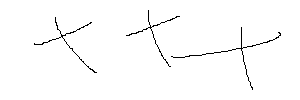
\includegraphics[width=0.35\textwidth]{unterschrift_rico}\vspace*{-0.35cm}
					\\
					\rule[0.5ex]{12em}{0.55pt} & \rule[0.5ex]{12em}{0.55pt} \\
					(Ort, Datum) & (Rico ) 
					\\

					
					  
					&
					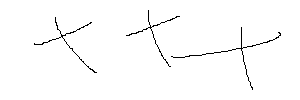
\includegraphics[width=0.35\textwidth]{unterschrift_henning}\vspace*{-0.35cm}
					\\
					 & \rule[0.5ex]{12em}{0.55pt} \\
					& (Henning ) 
					\\

					
					  
					&
					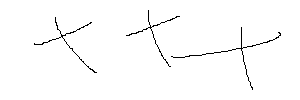
\includegraphics[width=0.35\textwidth]{unterschrift_julian.png}\vspace*{-0.35cm}
					\\
					 & \rule[0.5ex]{12em}{0.55pt} \\
					 & (Julian ) 
					\\



				\end{tabular*} \\
			\end{table}

\end{document}